\documentclass{ohm_project_description}

\projecttitle{Erkennung von Objekten mittels Semantischer Segmentierung}
\projectauthor{Labor für mobile Robotik}
\projectdate{2025}

\begin{document}

\maketitle
\thispagestyle{fancy}

\vspace*{-2.5cm}
\begin{figure}[h!]
    \centering
    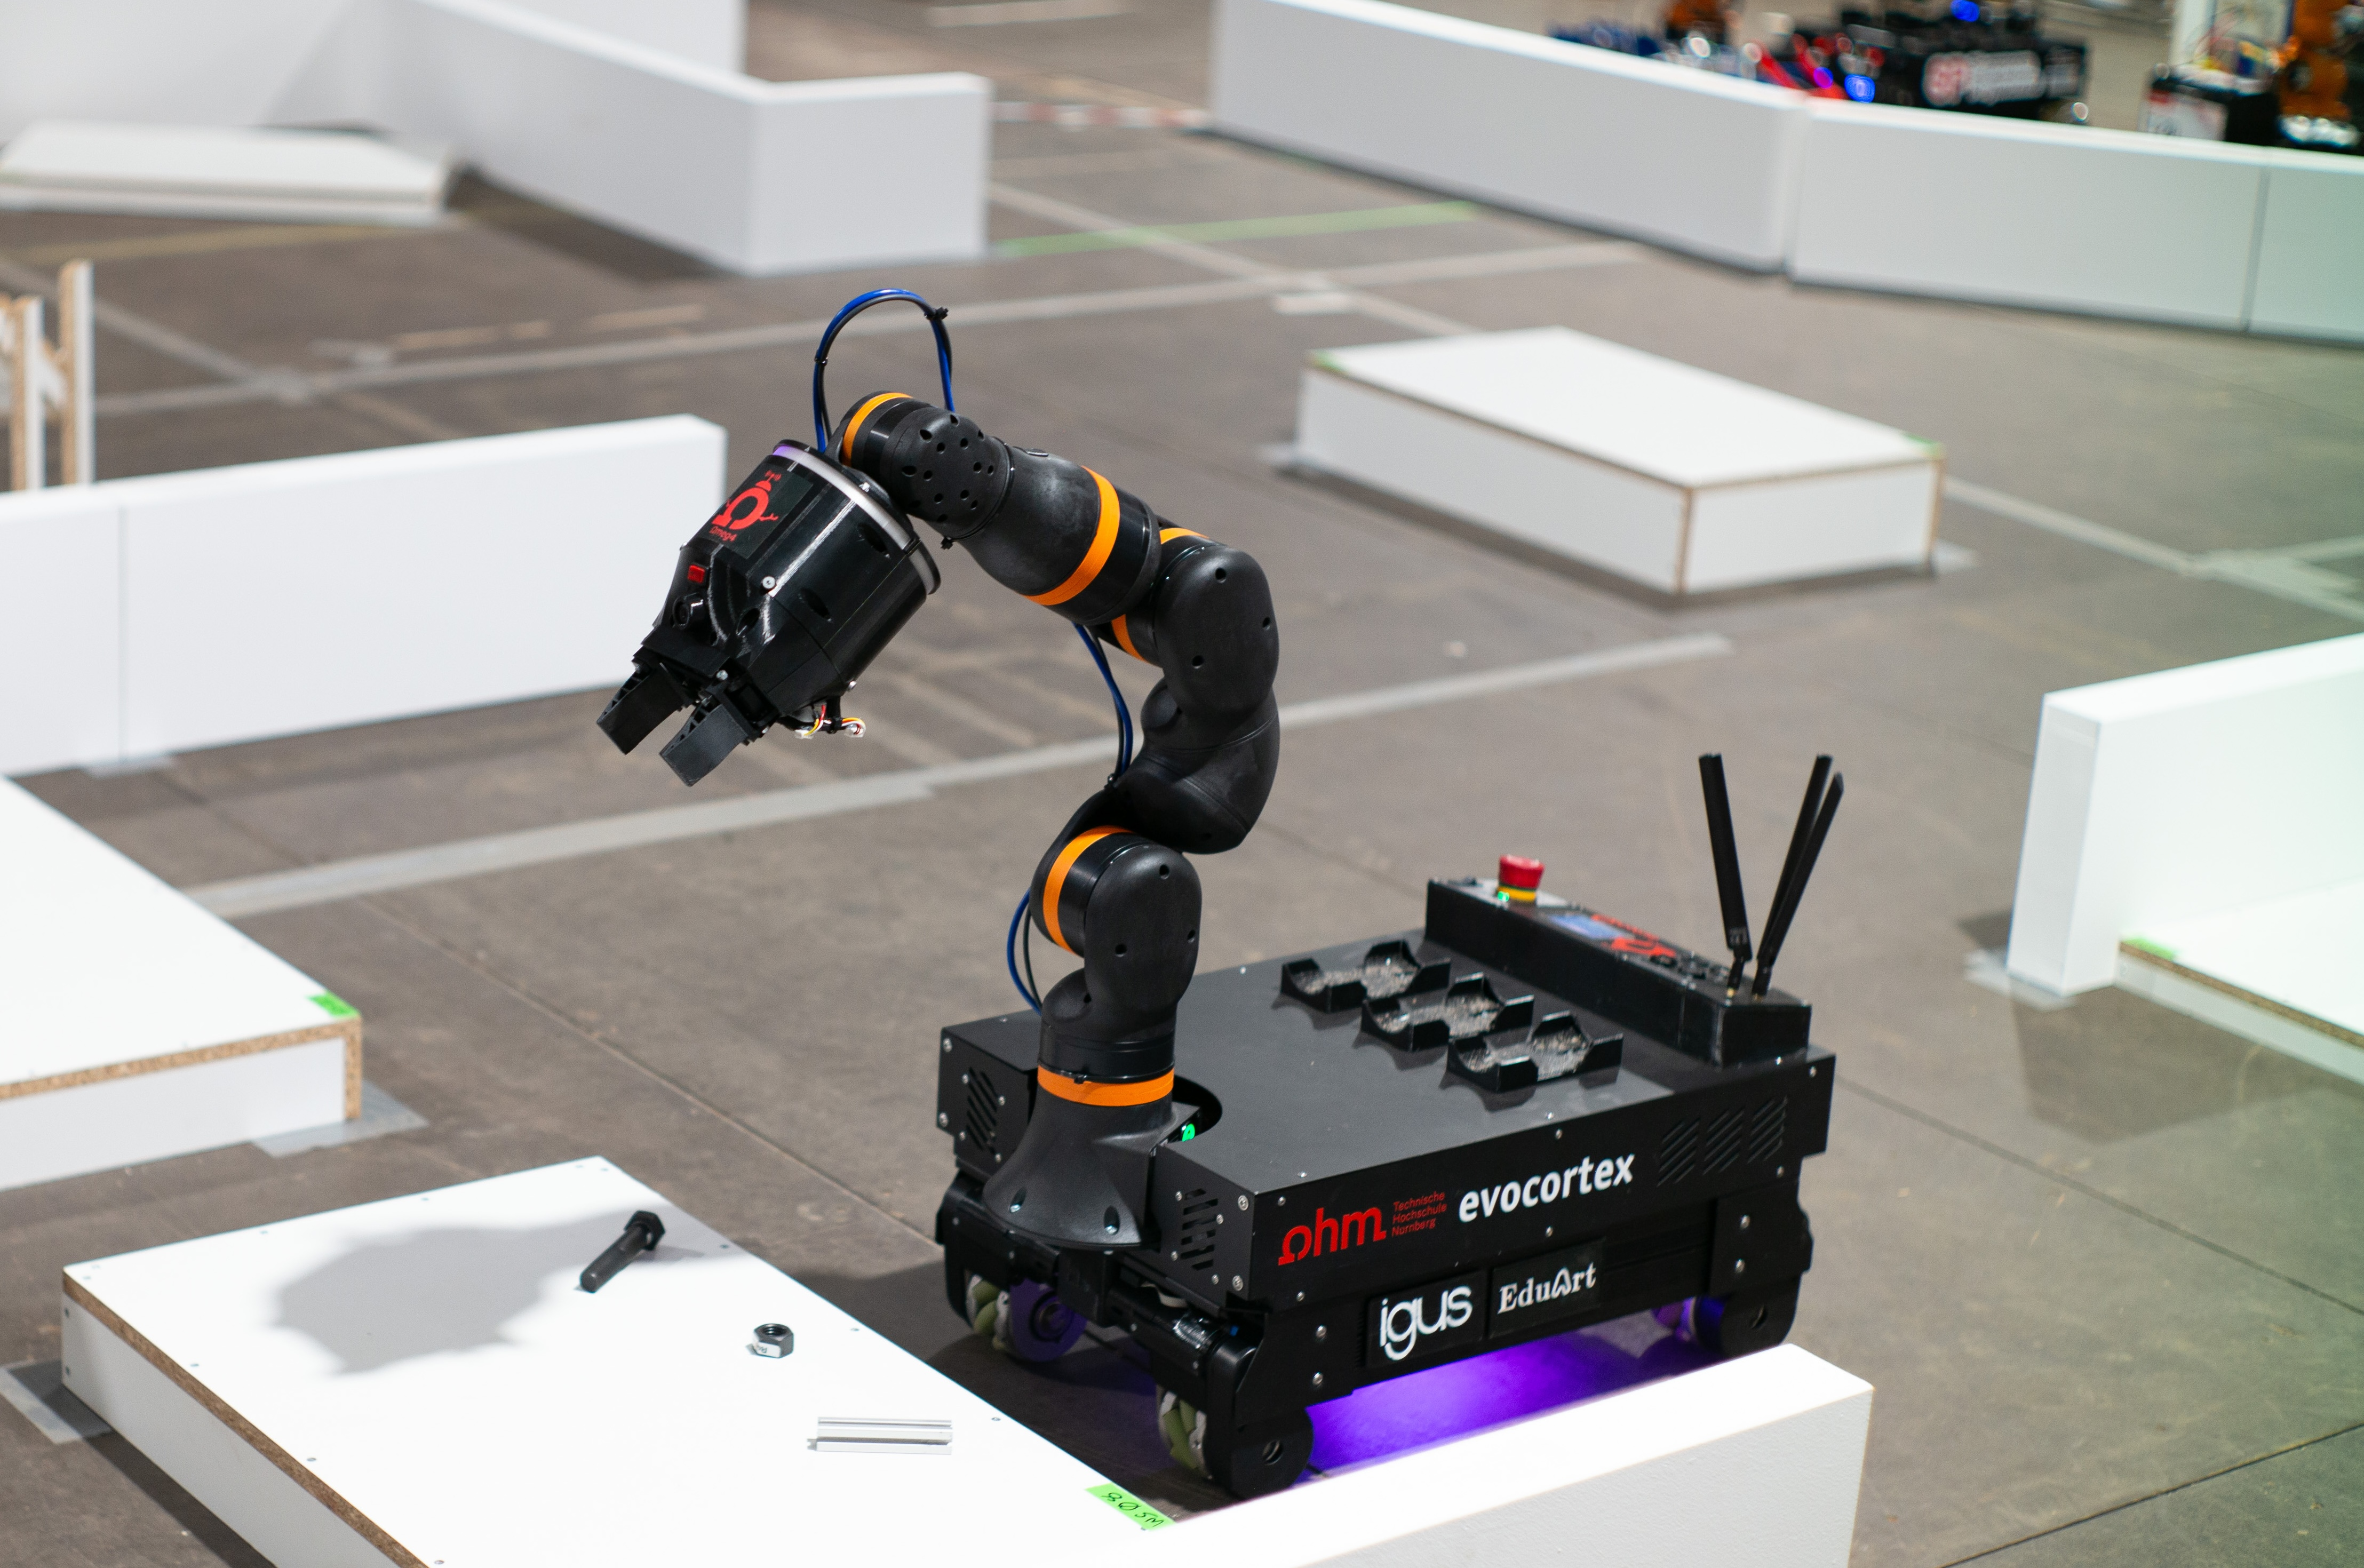
\includegraphics[height=4cm]{img/atwork.jpg}
\end{figure} 


Das Team \textbf{AutonOhm} des Labors für Mobile Robotik nimmt seit vielen Jahren erfolgreich am RoboCup Industrial @Work Wettbewerb teil. Ziel dieses Wettbewerbs ist es, einen mobilen Roboter zu entwickeln, der sich selbstständig in einer Arena zurechtfindet und vordefinierte Aufgaben der Form "Transportiere Gegenstand A von Tisch B zu Tisch C" durchführt. Für diese Aufgaben ist ein komplexes Gesamtsystem aus \emph{Lokalisierung}, \emph{Wahrnehmung}, \emph{Planung} und \emph{Steuerung} notwendig. Es bietet daher für interessierte Studierende neben einer Vielzahl von spannenden Themen im Bereich der mobilen Robotik auch die Möglichkeit, praxisnah an einem \emph{echten} Robotersystem zu arbeiten.

Ein wichtiger Teil des Systems ist die Erkennung von zu greifenden Objekten mittels einer Kamera. Aktuell werden Objekte in Form von rechteckigen Boundingboxen detektiert. Bei dieser Arbeit geht es darum, ein Erkennungssystem mittels semantischer Segmentierung, also dem pixelgenauen Klassifizieren von Bildinhalten, umzusetzen. Dies soll präziseres Greifen von Objekten ermöglichen. 

Engagement und Mitarbeit im studentischen Team Autonohm sind ausdrücklich erwünscht! Es besteht die Möglichkeit, im Rahmen der Arbeit an nationalen und internationalen Wettbewerben teilzunehmen.

\section*{Arbeitspakete}
\begin{itemize}[leftmargin=0.5cm]
    \setlength\itemsep{.1em}
    \item Erweitern der bestehenden Pipeline zur Erzeugung von synthetischen Trainingsdaten
    \item Ggf. erstellen von echten Trainingsdaten
    \item Recherche und Implementierung eines geeigneten Modells für semantische Segmentierung 
    \item Training und Validierung mit den spezifischen Daten für die RoboCop @Work Objekte
    \item (optional) Integration und Demonstration auf dem Robotersystem 
\end{itemize}

\section*{Voraussetzungen}
\begin{itemize}[leftmargin=0.5cm]
    \setlength\itemsep{.1em}
    \item Grundkenntnisse in einer höheren Programmiersprache (z.B. Python, C++)
    \item Grundkenntnisse in Deep Learning und Bildverarbeitung
    \item (optional) Grundkenntnisse in ROS
\end{itemize}

\vspace{0.5cm}
Das Thema kann nach Abstimmung als Bachelor- oder Masterarbeit bearbeitet werden, sowie als Projektarbeit. 


\vfill
\textcolor{ohm_red}{\rule{\linewidth}{0.4mm}}
\textbf{\textcolor{ohm_red}{Labor für mobile Robotik}} \\
\begin{tabular}{@{}ll}
\textbf{Betreuer:} & Prof. Dr. Enrico Schröder \\
\textbf{E-Mail:}   & \href{mailto:enrico.schroeder@th-nuernberg.de}{enrico.schroeder@th-nuernberg.de} \\
\end{tabular}

\end{document}